%!TEX root = uist14.tex
\section{Applications}
\label{sec:applications}

\ben{We may need to add some discussion of applications}.

Head orientation targeting can enable a wide range of context-aware applications. We implement one particular demonstrative application: a universal smart appliance controller. Users select a smart device (e.g., light fixture, TV, or home appliance) with Glass --- upon confirming the selection, an appliance-specific UI is shown on the user's near-eye display, and they can control the application (without having to continually look at it) through their device touchpad.

We implemented a prototype of this remote controller for three physical devices: a lamp and fan that could be switched on or off, and a smart TV control with playback, volume and navigation controls (see Figure~\ref{fig:smart-home}). We switched discrete appliances using relays, and implemented the smart TV with a laptop connected to a 30\inch{} display. User interfaces for each were pre-defined in our application. 

We set the devices up in a simulated living room environment and invited 14 users to step through a predefined set of tasks to control the appliances at a distance. 

%The huge benefit using head orientation is to solve two challenges that exist in most commercial list-based solutions -- {\em naming} and {\em scoping}. First, assigning clear names is non-trivial. Especially in shared spaces, the person trying to control the device might not be the one that named it - e.g., while an office building manager may know what ``Light 4 in area E'' corresponds to, an occupant may not. Second, without a method of scoping selection to automatically filter non-relevant devices, paging though long lists of names or navigating hierarchies becomes potentially more cumbersome than the physical action that the ``convenient'' software solution was meant to replace. Our head-orientation based interaction elegently solves these two problems.

%In order to control a smart appliance, the user performs a physical target selection (scan, refine and confirm) first and then the appliance-specific UI will be shown in the near-eye display. 

\begin{figure}[t]
\centering
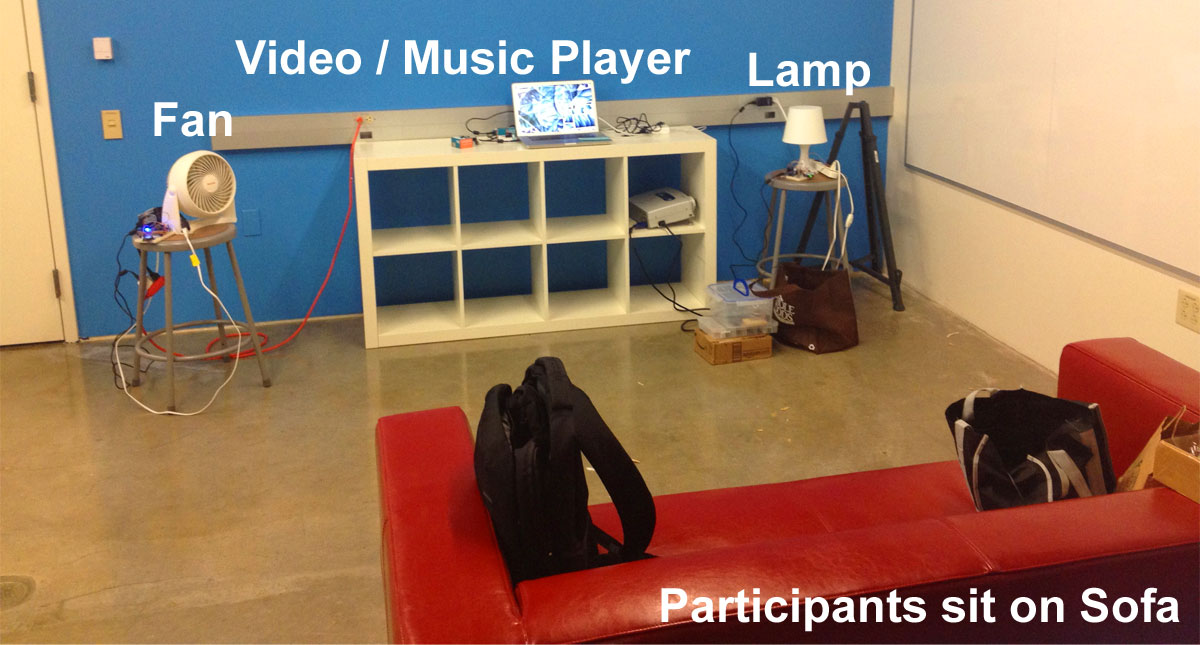
\includegraphics[width=1\columnwidth]{figures/smarthome-scenario.pdf}
\caption{In the smart home scenario, we have built three smart appliances for a user experience study. The interface supports both simple on/off appliances (lamp or fan) and multi-functional appliances (TV, for example).}
\label{fig:smart-home}
\end{figure}

%To assess the usability of such applications when the novel interaction scheme is added, we have built a few smart appliances (including a fan, a lamp and a TV, Figure~\ref{fig:smart-home}) and asked 14 participants to work through a concrete smart home scenario. The fan and lamp are relatively dumb and only support turning-on and turning-off. The smart TV provides control capability of switching the channels and adjust the volumn, as well as pause/play. From this study, we report some of the qualitative results to strength our motivation for the head-orientation interaction.

All participants successfully completed the list of tasks. They commented positively on the universal remote control functionality (e.g., \studyquote{I didn't have to search for different remote controllers for different appliances}) and stated it was easy to target and connect to appliances, in line with the findings of the previous study procedure. Participants saw potential benefits of the device for families; one user remarked that he could imagine people using the system \studyquote{while keeping an eye on their children at the same time}.

\sean{here are some parts I can think of to add to this section, feel free to refine/elaborate/remove.} 
\bjoern{1 is problematic - because it sounds like that the head worn device is in the end not worth it and you should just use your phone, even if it takes longer. I'm not sure we can confidently say something about museums or body shops - this sounds speculative. Needs section needs to be rephrased., e.g. as in: Our solution succeeds at X because of Y. This suggests that future applications in domains like Z could be especially promising.}
\changes{During our study, we learned a few things. (1)Our soulution works best on simple applications such as on/off or volume up/down controls. For more complicated controls, we suggest to use a hybrid solution in which HOBS completes the target selection process and seamlessly transfer information to user's smartphone and triggers corresponding app.  (2)Our solution excels at tasks where the user needs to focus primarily on the objects and the information provided by the near-eye display is only supportive, for example, museums or automobile body shops. (3)Our soulution also works well for roles whose hands are constantly occupied from using handheld devices, e.g. chefs.}
%% I feel like we should mention a bit about the interaction complexity. But that's a bit out of the scope of this paper.
%% Participants rated the ease of control of particular appliances differently. Ease of use ratings were higher for the lamp and fan which had simple, discrete on/off actions, and lower for the more complex movie player (see Figure~\ref{fig:smarthome-likert}). Multiple participants remarked that the difficulty was based on the affordances of Glass: \studyquote{Most of the difficulty I had with Glass came from having to navigate the interface on the tiny screen with the touch pad}. The screen size and (largely) 1D input put a limit on the complexity of interfaces that can be presented. As one participant remarked: \studyquote{[The media player] does not seem to be more efficient than a tablet device.} The difficulty can also partly be ascribed to our interaction design, which required one finger swipes to switch between parameters and two finger gestures for adjusting parameters --- it was hard for users to exert fine control over two-finger swipes. In addition, users did not always remember these mappings as they are not yet part of a standard gesture vocabulary.

%\subsection{Attention Tracking}
%\label{sec:attention-tracking}

%The second tier of applications enabled by our system is an implicit use of users' head orientation. One sample application is to obtain a personal statistics. Nowadays, we are surrounded by all sorts of screens, and many people's job requires them to stare at the monitors for the whole day. 
% citation needed, take a look at this one: E-Readers and Visual Fatigue, http://www.ncbi.nlm.nih.gov/pmc/articles/PMC3873942/
%Knowing how much time you have spent in front of the screen is definitely useful, and the application can be built to remind the user to take a break whenever a certain time threshold is reached.

%% We might be lacking evidence, but let me just write down the draft first.
%Our system enables a flexible and easy-to-use tracking of users' attention without knowing the map. Therefore, it's suitable to be deployed in large museums (even when the exihibits positions are adjusted constantly). Then such attention tracking will facillitate many social science studies. Previous solutions are either using RFID \cite{Hsi:2005:REV:1081992.1082021} or video taping % this is a cv of Adam who has worked on video analysis http://www.exploratorium.edu/vre/cvs/ak_cv.pdf. 
%However, head orientation is a better approximation of attention rather than proximity. By placing our tracking devices in the environment, we can easily get a more accurate profiling of users intention.

%\subsection{Indoor Positioning}
%\label{sec:indoor-positioning}

%There is one category of indoor positioning which is based on angle of arrival. Traditional approaches on indoor positioning are based on fingerprinting or triangulation, which is known to be bad due to multi-path effect for indoor environment. With our system, using the adjacent mapping calibration we can figure out the position of the targets in a room, and then based on a new sample, we can estimate a user's position with some simple math.



%%% Local Variables: 
%%% mode: latex
%%% TeX-master: "uist14"
%%% End: 
